\section{Implementation}\label{impl}
This section overviews the implementation of SCache -- a distributed in-memory shuffle data storage system with a DAG co-scheduler. Here we use Spark as example of DAG framework to illustrate the workflow of shuffle optimization. We will first present system overview in Subsection \ref{arch} while the following two subsections focus on the two constraints on memory management.

\subsection{System Overview}\label{arch}
SCache consists mainly three components: A distributed in-memory shuffle data storage system, a DAG co-scheduler and the daemon inside Spark. As shown in Figure \ref{fig:arch}, for the in-memory storage system, SCache employs the legacy master-slaves architecture like GFS\cite{gfs}. The master node of SCache coordinates the shuffle blocks globally with application context from Spark. The coordination provides two guarantees: (a)store data in memory before tasks start and (b)schedule data on-off memory with all-or-nothing property and context-aware-priority constraints to benefit all jobs. The worker node reserves memory to store blocks and bridges the commuication between Spark and SCache. The co-scheduler is dedicated to pre-schedule reduce tasks with DAG information and enforce the scheduling result to Spark.

When a Spark job starts, the DAG will be first generated. Spark DAG scheduler recursively visits the dependencies from last RDD. While going forward to the beginning, the DAG computing pipeline will be cut off if a RDD has one or more shuffle dependencies. These shuffle dependencies among RDDs will then be submitted through RPC call to SCache master by a daemon process in Spark driver. For each shuffle dependency, the shuffle ID(an integer generated by Spark), the type of partitioner, the number of map tasks and the number of reduce tasks are included in the RPC call. The SCache master will store the metadata of one RPC call as a set of shuffles scheduling unit. If there is a specialized partitioner, such as range partitioner, in the shuffle dependencies, the daemon will insert a sampling program in the host RDD. This sampling application will be scheduled ahead of that host RDD. We will elaborate the sampling procedure in the Section \ref{sampling}.

For the hash partitioner, when a map tasks finishes computing, the SCache daemon process will transfer the shuffle map output from Spark executor to the reserved memory through memory copy. 
At the same time, the map task will end and the slot will be released after the memory copy without the shuffle map output persistence. 
When the shuffle map output is received, the SCache worker will then notify the master of the block belonging information with the reduce size distribution in this block (see map output in Figure \ref{fig:shuffle}). 
If the collected map output data reach the observation threshold, the SCache co-scheduler will then run the scheduling algorithm \ref{mhminheap} (for multiple shuffle dependencies) and \ref{hminheap} (for single shuffle dependency) to pre-schedule the reduce tasks and then broadcast the scheduling result.
The pre-fetching of shuffle data starts as soon as each worker receives the scheduling results. 
More specifically, each worker will filter the reduce tasks ID that will be launch on itself. 
When a map task finishes, each node will receive a broadcast message. The pre-fetch process will be triggered to start fetching shuffle data from the remote SCache worker. After the blocks of shuffle map output are transferred, the SCache worker will flush these blocks to disk to memory space and maintain fault tolerance of Spark. 

Before the reduce stage starts, Spark DAG Scheduler will first generate a task set for this stage with different locality levels --- \textit{PROCESS\_LOCAL, NODE\_LOCAL, NO\_PREF, RACK\_LOCAL, ANY}.
To enforce SCache pre-scheduled the tasks --- node mapping, we insert some lines of codes in Spark DAG Scheduler.
For RDDs with shuffle dependecies, Spark DAG scheduler will consult SCache master to get the preferred node for each partition and set \textit{NODE\_LOCAL} locality level on corresponding tasks. 

When the scheduled reduce tasks start, the shuffle input data can be fetched from reserved memory in SCache worker through daemon process. As soon as the data is consumed by reduce task, it will be flushed to the disk.

\subsubsection{Reservior Sampling}\label{sampling}
If the submitted shuffle dependencies contain a range partitioner or a customized non-hash partitioner, the SCache master will send a sampling request to daemon in Spark driver. The daemon then insert sampling job with corresponding RDD. This sampling job uses a reservoir sampling algorithm\cite{reservoir} on each partition of RDD. For the sample number, we set the size equals to $3 \times number\ of\ partitions$ for balancing overhead and accuracy (it can be tuned by configuration). The sampling job randomly select some items and performs a local shuffle with partitioner (see Figure \ref{fig:sample}). At the same time, the items number of this partition is counted as the weight. These sampling data will be aggregated by $reduce\ ID$on SCache master. The prediction of reduce size can be easily computed by equation \ref{equationsample}. After the prediction, master will call algorithm \ref{mhminheap} and \ref{hminheap} to do the scheduling. 

\begin{figure}
	\centering
	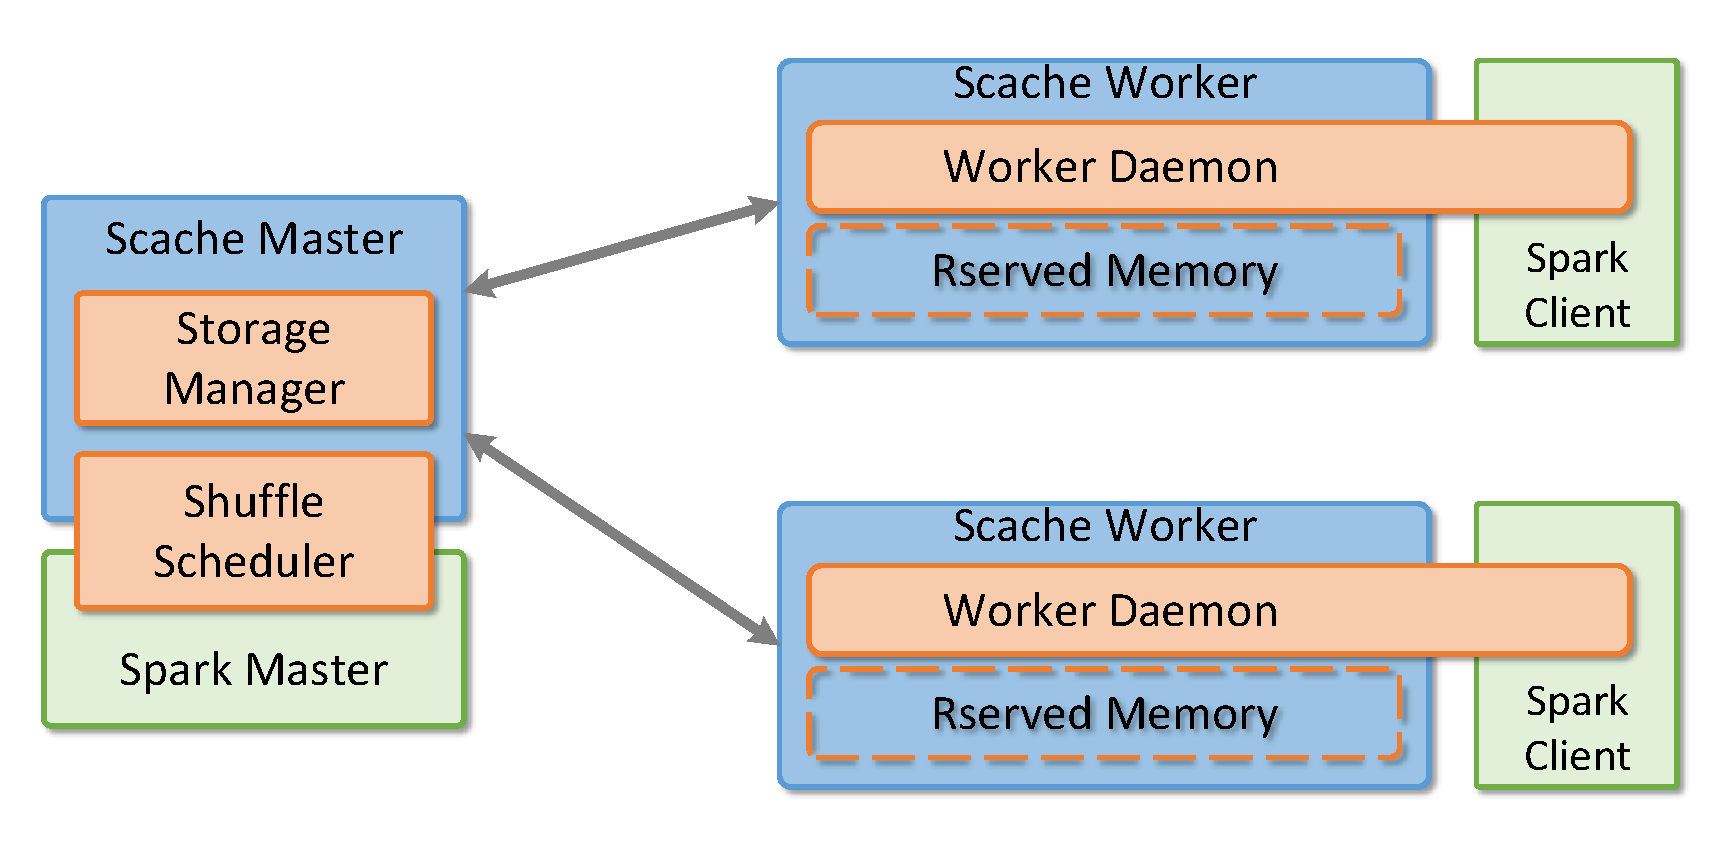
\includegraphics[width=0.9\linewidth]{fig/arch}
	\caption{SCache Architecture}
	\label{fig:arch}
\end{figure}
\begin{figure}
	\centering
	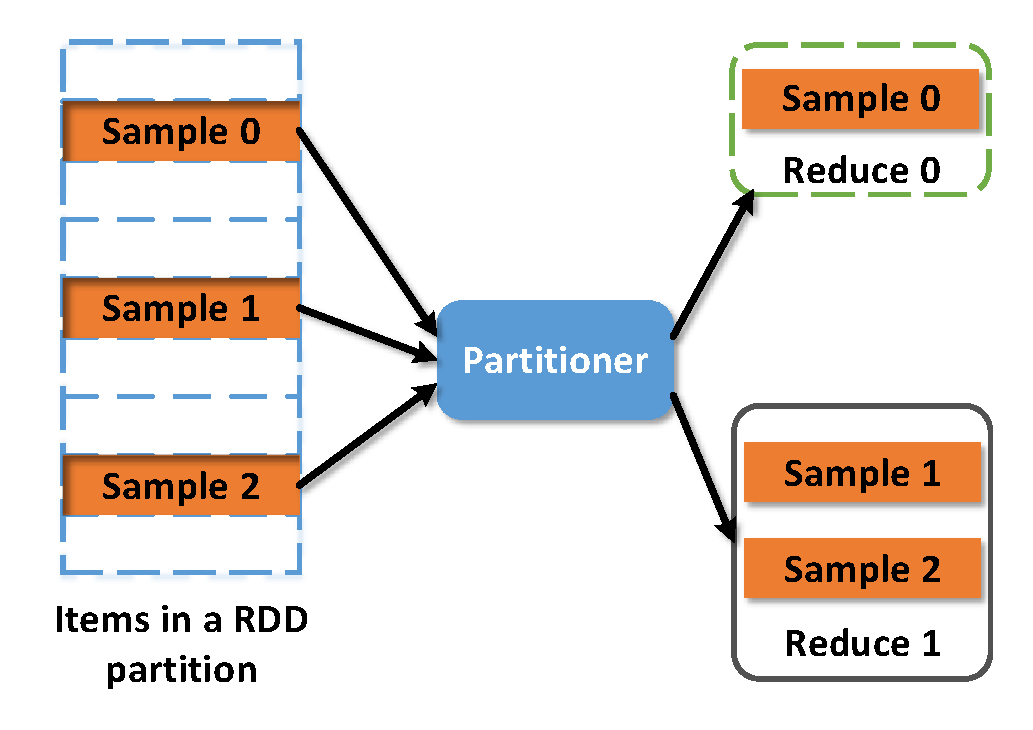
\includegraphics[width=0.7\linewidth]{fig/sample}
	\caption{Reservoir Sampling of One Partition}
	\label{fig:sample}
\end{figure}

\subsection{Memory Management}
As mentioned in section \ref{observation}, despite the shuffle size is small enough to be fitted in memory, unfortunately, the probability of memory exceeded is still exist. 
When the cached data meet the limitation of reserved memory, SCache flushes some of them to the disk temporarily. 
And re-fetch them as soon as some cached shuffle blocks is consumed or pre-fetched. To achieve maximum overall improvement, SCache leverages two constraints to manage the in-memory data --- all-or-nothing and context-aware-priority.

\subsubsection{All-or-Nothing Property}
Memory cached shuffle can speed up the reduce task execution. But this acceleration of single task is necessary but unsufficient for a shorter stage completion time. Base on the observation that in most cases one single stage contains multi-rounds of tasks from section \ref{multi}, if one of the task misses a memory cache and exceeds the original bottleneck of this round, that task will become the new bottleneck and might further slow down the whole stage. PACMan\cite{pacman} has also proved that for multi-round stage/job, the completion times improves in steps when $n\times number\ of\ tasks\ in\ one\ round$ of tasks have data cached simultaneously. Therefore, the memory cache of shuffle data need to match at least all tasks in a running round. We refer to this as the all-or-noting property. 

According to all-or-nothing property, SCache master leverages the pre-scheduled results to determine the bound of each round, and then use this as the minimum unit of storage to manage the reserved memory globally.
That is, the storage unit number equals to the number of task round for a shuffle schedule unit.
For those incomplete unit, SCache will mark them as the lowest priority.
% Following the all-or-noting constraint can maximum the improvement in stage completion time by using reserved memory efficiently.

\subsubsection{Context-Aware-Priority Property}
When the size of cached shuffle data exceeds the reserved memory, SCache should decide which of these should be flushed to disk according to the priorities of each storage unit. SCache master first searches if there is an incomplete unit and flush all blocks belonging to the unit to disk cluster-widely. 

But what if all the units are completed in the cluster? Traditional cache replacement schemes, such as MIN\cite{min}, only maximize cache hit ratio without considering the application context in DAG computing. 
Directly appyling them might easily violate all-or-nothing constraint.
In addition, since the cached shuffle blocks are only read exactly once (without failure), the hit ratio is actually meaningless in this scenario.
To decide the priorities among units, SCache makes decision in two dimensions -- \textit{inter-shuffle units} and \textit{intra-shuffle unit}. 
\begin{itemize}[noitemsep]
	\item Inter-shuffle units: SCache master follows the scheduling scheme of Spark to determine the inter-shuffle priority. For a FAIR scheduler, Spark balances the resource of among task sets, which leads to a higher priority for those with more remaining tasks. More remaining tasks a stage implies more storage units left unconsumed. So SCache sets priorities from high to low to each shuffle units in descending order of remaining storage units. For a FIFO scheduler, Spark schedules the task set that is submitted first. So SCache sets the priorities according to the submit time of each shuffle unit.
	\item Intra-shuffle unit: SCache also needs to decide the priority among storage units inside a shuffle unit. Referring to the task scheduling inside a task set of Spark, the tasks with smaller ID will be scheduled at first under one locality level. Based on this, SCache can assign the storage unit with larger tasks ID with lower priority.
\end{itemize}
In a word, SCache selects the shuffle unit with lowest priority and evicts the storage units by intra-shuffle priority.



% \subsubsection{Fault Tolerance}
% To prevent the machine failure in cluster leading to inconsistency SCache, the master node will log the meta data of shuffle register and scheduling on the disk. Since we remove the shuffle transfer from the critical path of DAG computing, the disk log will not introduce extra overhead to the DAG framworks. Note that the master can be implemented with Apache ZooKeeper\cite{zookeeper} to provide constantly service to DAG framework.  
% At the same time, every work node will send a heartbeat to master to report status. If a failure of work node is detected, the master will the do a simple re-schedule. For those scheduled shuffle units, the master assgins the tasks to other workers with more lightweight workload evenly. Then the new assigned worker will fetch the data again. For the incomplete in memory map blocks on the failure node, SCache simply ignore them since DAG framework will schedule the failure map tasks on another node.
